% ============================================================
% CHAPTER: PROTOTYPE
% ============================================================

\chapter{Prototype}

We developed an interactive web application for predicting depression levels and emotional states using voice recordings. The system includes a user-friendly interface for voice input, real-time audio playback, and seamless navigation. It leverages machine learning models to analyze audio data and provide accurate predictions.

The home page provides an overview and entry point to begin the assessment.

\begin{figure}[htbp]
    \centering
    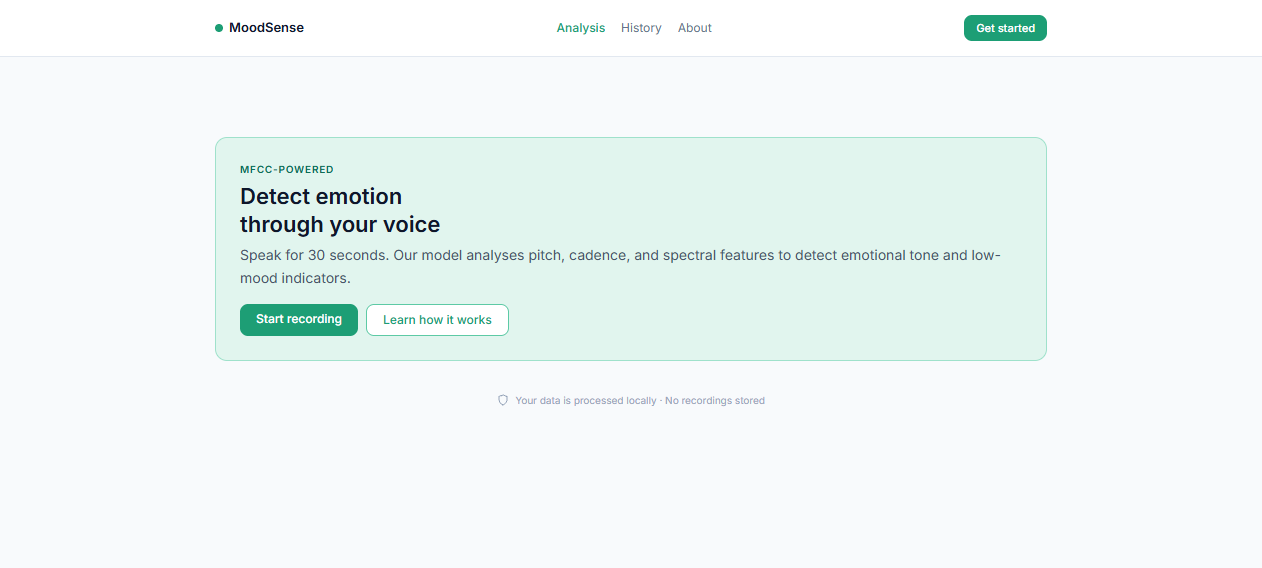
\includegraphics[width=0.8\textwidth]{media/landing-page.png}
    \caption{Home page of the stress detection application}
    \label{fig:landing}
\end{figure}

Users record their voice responses through the assessment interface, with controls for starting, stopping, and playing back recordings. These voice inputs are processed to predict emotional states and stress levels.

\begin{figure}[htbp]
    \centering
    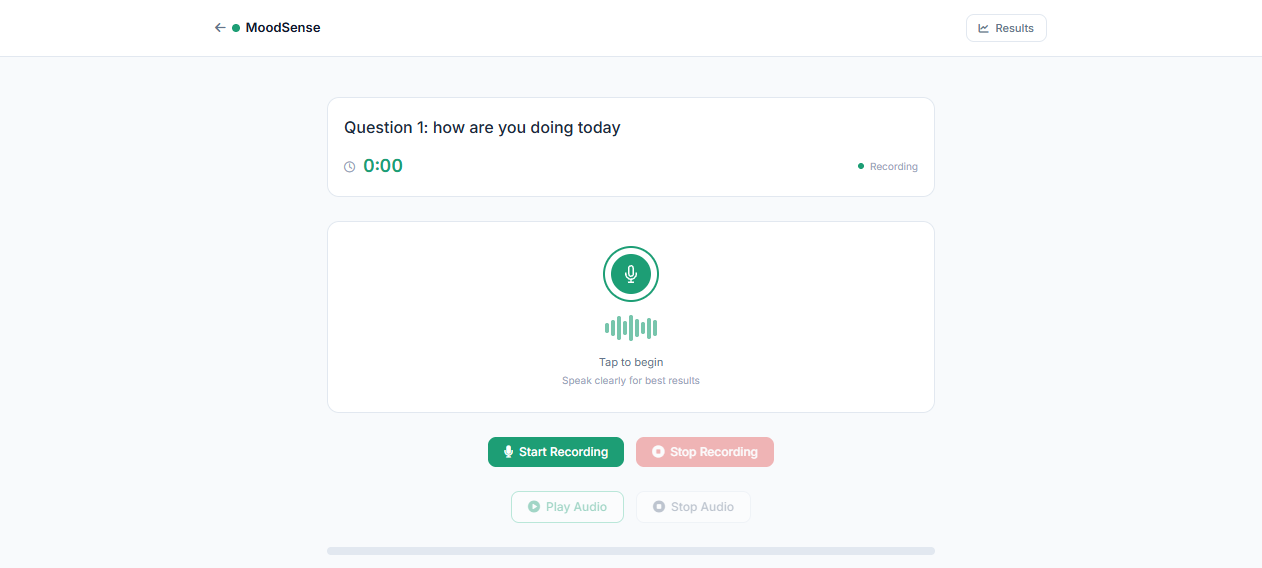
\includegraphics[width=0.8\textwidth]{media/question-page.png}
    \caption{Voice recording interface for assessment}
    \label{fig:recording}
\end{figure}

The results page displays predicted emotions, depression levels, and visual charts generated from the ML analysis.

\begin{figure}[htbp]
    \centering
    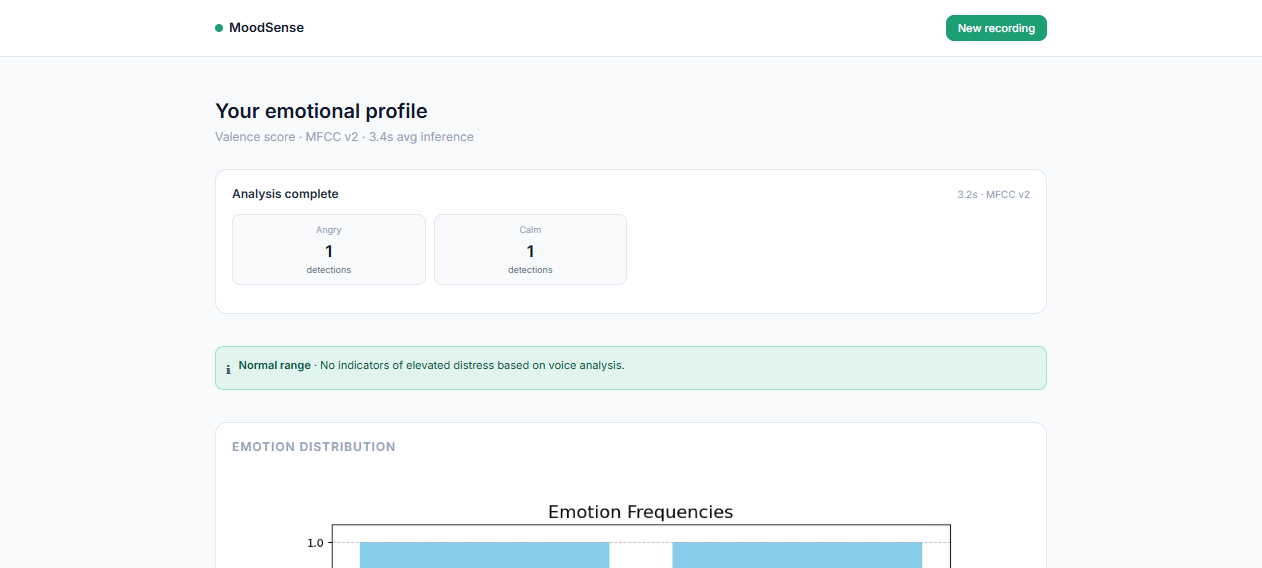
\includegraphics[width=0.8\textwidth]{media/results-page.png}
    \caption{Results page showing predictions and charts}
    \label{fig:results}
\end{figure}

The application flow consists of: (i) a landing page to begin the assessment, (ii) a voice recording interface for user responses, (iii) a backend that segments audio into 3-second clips for emotion detection and 2-minute chunks for depression analysis, and (iv) a results page displaying predicted emotions, stress levels, and visual insights. The prototype demonstrates the practical viability of using vocal analysis for mental health assessment, providing a foundation for future development and commercialization.
